\chapter{Zarovnávanie sekvencií}
\label{chap:alignment}

V~tejto kapitole si stručne popíšeme čo je to globálne a lokálne zarovnanie a ukážeme základné algoritmy na hľadanie globálneho a lokálneho zarovnania. Tieto algoritmy budeme neskôr modifikované používať pri našom riešení.

\section{Podobnosť sekvencií, sekvenčná homológia a zarovnanie}
V~prírode vznikajú evolúciou nové DNA sekvencie (ďalej len sekvencie) modifikáciou už existujúcich. Preto môžme často spozorovať podobnosť medzi neznámou sekvenciou a sekvenciou o~ktorej už niečo vieme. Ak zistíme podobnosti medzi sekvenciami, môžeme preniesť informácie o~štruktúre a/alebo funkcii na novú sekvenciu.

Podobné sekvencie, ktoré sa vyvinuli mutáciami zo sekvencie v~spoločnom predkovi sa nazývajú \textit{homologické} a pod pojmom \textit{hľadanie homológov} rozumieme hľadanie takých podobností, ktoré s~veľkou pravdepodobnosťou vznikli práve spoločnou evolučnou históriou.

%Na prvý pohľad rozhodnutie podobnosti dvoch biologických sekvencií nie je nič iné, ako rozhodnutie podobnosti dvoch textových reťazcov.
%--Tuto vetu tam nechceme--Mnoho metód analýzy biologických sekvencií je preto zakorenená v informatike, kde je už mnoho literatúry týkajúcej sa tejto problematiky.

%Vývoj sekvencií hromadí \textit{inzercie}, \textit{delécie} a \textit{substitúcie}, takže predtým ako môže byť vyhodnotená podobnosť, treba urobiť zarovnanie sekvencií. Preto je zarovnanie sekvencií veľmi dôležité.

Počas evolúcie dvoch homologických sekvencií nastane veľa \textit{inzercií}, \textit{delécií} a \textit{substitúcií}, preto predtým ako môžeme začať porovnávať sekvencie, ich musíme zarovnať tak, aby homologické časti sekvencií boli na rovnakom mieste v~zarovnaní. Substicúcie nastanú ak niektorá báza zmutuje, teda sa zmení na inú. Inzercie nastanú ak sa do sekvencie pridá nejaký súvislý úsek a delécie nastanú ak zo sekvencie vypadne súvislý úsek. Inzerciu a deléciu označíme spoločne pojmom indel. Indely v~sekvencii voláme aj medzery a označujeme pomlčkami. Pričom vo všeobecnosti ak máme medzeru v~jednej sekvencii, nevieme povedať, či ide o~deléciu v~tejto sekvencii, alebo inzerciu v~druhej.
\cite{durbin, skripta}

\begin{figure}[hbtp]
    \centering
    % 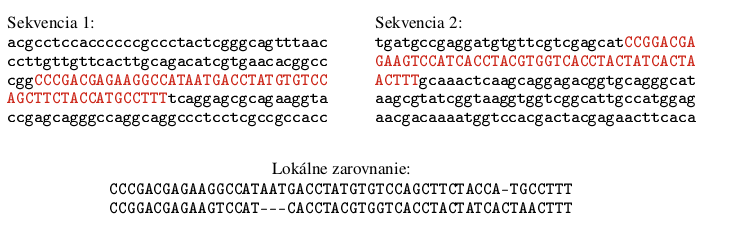
\includegraphics[width=.8\textwidth]{images/zarovnanie}
    \begin{subfigure}[m]{0.45\textwidth}
    \centering
    \begin{center}
    Sekvencia 1:
    \end{center}
    \begin{BVerbatim}[commandchars=\\\{\}]
gagacccgcctaggtgaatatttagcagc
gattaaataccacgta{\color{red}TATAAGGTGGACC}
{\color{red}GTTCCTCGAGAGGTTCTTCCGGCAATGAC}
{\color{red}GGCCAGAGCAAAAGCCACGT}gtaggactg
catacgcctctacgcctccactgacgcga
tgatgtggcgtggatctgtttgctcttgg
tataggtcacggagacggctggtactgat
cccttcgggagtaaaaatataatgaccat
ggcccaggcttcaggagggagttgtgcgg

    \end{BVerbatim}
    \end{subfigure}
    \qquad
    \begin{subfigure}[m]{0.45\textwidth}
    \centering
    \begin{center}
    Sekvencia 2:
    \end{center}
    \begin{BVerbatim}[commandchars=\\\{\}]
tgtacagcactgcaacgagcatctggggg
ttggttattccgatggcgctggacagcta
gcggacagtagttctcaggccttagtaga
aaggtgggaaccccc{\color{red}TATGAGGTCGACCG}
{\color{red}TTTCAGCGTGACTATAGACGTCATTGAAG}
{\color{red}CAATATACAGGAACACCACCT}acttagga
agggagttcggtgcagtaaagcattctta
cctcagggcacggtagagaacactacaac
cagaatagcaacgtgatgcggcgactctc

    \end{BVerbatim}
    \end{subfigure}
    \begin{center}
    Lokálne zarovnanie:
    \end{center}
    \begin{BVerbatim}
TATAAGGTGGACCGTT--------CCTCGAGAGGTTCTTCCGGCAATGGCCACGAGAGCAAAAGCCACGT
TATGAGGTCGACCGTTTCAGCGTGACTATAGACGTCATTGAAGCAATATACAGG------AACACCACCT
    \end{BVerbatim}
    \caption[Lokálne zarovnanie]{Dve sekvencie a ich lokálne zarovnanie. Veľkými písmenami a červenou farbou sú vyznačené zarovnané časti. V~zarovnaní sa nachádzajú zhody, nezhody a medzery v~oboch sekvenciách}
    \label{fig:alignment_example}
\end{figure}

\section{Párové zarovnávanie}
Párové zarovnávanie je základná úloha zarovnávania sekvencií, kde sa k~sebe zarovnávajú dve sekvencie. V~tejto práci sa budeme zaoberať len párovým zarovnávaním.

Kľúčové problémy sú:
\begin{enumerate}
\item Aké typy zarovnávania by sme mali uvažovať
\item Skórovací systém, ktorý použijeme na ohodnotenie zarovnania a trénovanie
\item Algoritmus, ktorý použijeme na hľadanie optimálneho alebo dobrého zarovnania podľa skórovacieho systému
\item Štatistická významnosť zarovnania.
\end{enumerate}

\cite{durbin}

\section{Typy zarovnaní}
Základné typy zarovnaní sú \textit{Globálne zarovnanie} a \textit{Lokálne zarovnanie}.
\begin{df}[Globálne zarovnanie]
Vstupom sú dve sekvencie $X = x_1x_2\dots x_n$ a $Y = y_1y_2\dots y_m$
Výstupom je zarovnanie celých sekvencií $X$ a $Y$.
\end{df}

\begin{df}[Lokálne zarovnanie]
Vstupom sú dve sekvencie $X = x_1x_2\dots x_n$ a $Y = y_1y_2\dots y_m$
Výstupom je zarovnanie nejakých podreťazcov $x_i\dots x_j$ a $y_k\dots y_l$ sekvencií.
\end{df}
V~praxi sa väčšinou snažíme nájsť zarovnania s~najvyšším skóre.
\cite{skripta}

\section{Skórovacie systémy}
Takmer všetky metódy zarovnania hľadajú zarovnanie dvoch reťazcov na základe nejakej \textit{skórovacej schémy}. Skôrovacia schéma je metóda, ktorou priradíme zarovnaniu skóre -- zvyčajne čím väčšie skóre, tým realistickejšie zarovnanie by to malo byť.
Skórovacie schémy môžu byť veľmi jednoduché, napr. $+1$ za \textit{zhodu} a $-1$ za \textit{nezhodu} a \textit{medzeru}.
Ak chceme mať schému, kde biologicky najkorektnejšie zarovnanie má najvyššie skóre, musíme vziať do úvahy, že biologické sekvencie majú evolučnú históriu, 3D štruktúru a mnohé ďalšie vlastnosti obmedzujúce ich evolučné procesy. Skórovací systém, ktorý by uvažoval všetky tieto faktory, by bol veľmi zložitý, preto sa používajú jednoduchšie, ktoré zanedbávajú veľa faktorov.
\cite{durbin}

\subsection{Skórovacie matice}
Skoro vždy však chceme rôzne zhody a nezhody skórovať rôzne - nie len všetky zhody $+1$ a nezhody $-1$.
Skóre môže záviseť od toho aké bázy sú v~danom stĺpci zarovnania. Na to sa používa \textit{skórovacia matica} (obr. \ref{fig:scoringmatrix}), kde máme definované skóre pre každú dvojicu. Skórovacie matice sa využívajú aj pri zarovnávaní proteínov, kde niektoré dvojice majú podobné chemické vlastnosti
\cite{durbin, skripta}.
Môžme mať aj afínne skôrovanie medzier, kde máme iné skóre za začatie medzery ako za predĺženie medzery. O~tom si popíšeme v~sekcii \ref{subsec:affine-gap-scoring}
Iným typom skórovacej schémy je napríklad \textit{párový skrytý markvovský model} (viac v~sekcii \ref{sec:hmm-alignment})

\begin{figure}[hbtp]
    \centering
    \begin{tabular}{r|ccccc}
    & A~& C & G & T & -\\
    \hline
    A~& 6 & -1 & -2 & -1 & -3\\
    C & -1 & 5 & -3 & -2 & -4\\
    G & -2 & -3 & 5 & -2 & -2\\
    T & -1 & -2 & -2 & 6 & -1\\
    - & -3 & -4 & -2 & -1 & $\infty$\\
    \end{tabular}
    \caption[Skórovacia matica]{Ukážka skórovacej matice. Všimnime si, že môžu byť rôzne skóre aj za jednotlivé zhody, nezhody alebo medzery.}
    \label{fig:scoringmatrix}
\end{figure}

\section[Algoritmy]{Algoritmy na hľadanie zarovnaní}
Pre danú skórovaciu schému potrebujeme algoritmus, ktorý nájde optimálne zarovnanie dvoch sekvencií.
Budeme uvažovať zarovnávanie s~medzerami. Medzery používame na znázornenie inzercie alebo delécie\footnote{vo všeobecnosti nevieme povedať, či ide o~inzerciu v~jednej sekvencii alebo deléciu v~druhej sekvencii}. Na označenie medzier používame pomlčku {\tt'-'} a medzeru do sekvencie medzi dve bázy pridáme tak, že medzi dve bázy napíšeme jednu alebo viac pomlčiek -- počet pomlčiek zodpovedá počtu medzier a teda aj počtu báz, ktoré má na danom mieste jedna sekvencia navyše oproti druhej. Do sekvencie môžeme pridať ľubovoľne veľa medzier (pričom nemôžeme mať dve pomlčky v~jednom stĺpci), aby sme dosiahli lepšie skóre. Pre dve sekvencie dĺžky $n$ existuje
$$ {2n \choose n}  = \frac{(2n)!}{(n!)^2} \simeq \frac{2^{2n}}{\sqrt{\pi n}} $$
možných globálnych zarovnaní. \cite{durbin} Pre dlhšie sekvencie nie je možné enumerovať všetky a vybrať tú s~najlepším skóre.

Algoritmy na hľadanie zarovnaní využívajú \textit{dynamické programovanie}.
Často sa používajú aj rôzne heuristiky na urýchlenie výpočtu.
My sa zaoberať algoritmami využívajúcimi heuristiky nebudeme. Pre rôzne typy zarovnaní a skórovacie schémy máme rôzne algoritmy zarovnávania.
\cite{durbin, skripta}

\subsection{Algoritmus pre globálne zarovnanie: Needelman-Wunch}
\label{subsec:global-alignment}
Máme dané dve sekvencie $X = x_1x_2\dots x_n$ a $Y = y_1y_2\dots y_m$, budeme zarovnávať všetky znaky sekvencie $X$ a všetky znaky sekvencie $Y$.
Definujeme si jednoduchú skórovaciu tabuľku kde $s(x, y)$ bude udávať skóre pre danú dvojicu báz (napr. $+1$ za zhodu, $-1$ za nezhodu) a za každú medzeru budeme dávať penaltu $-d$.

%Idea je nasledovná - Nech máme optimálne zarovnanie dĺžky $n$. Zarovnanie dĺžky $n+1$ vieme vyrobiť 3 spôsobmi. Buď pridáme $(x_i,y_j)$, alebo $(x_i,-)$, alebo $(-,y_j)$, kde $i,\ j$ sú indexy prvej nepoužitej bázy v $X$ resp. $Y$. Možnosť s najlepším skore nám dá optimálne zarovnanie dĺžky $n+1$.

\begin{figure}[htp]
    \centering
    \begin{subfigure}[m]{0.5\textwidth}
    \centering
    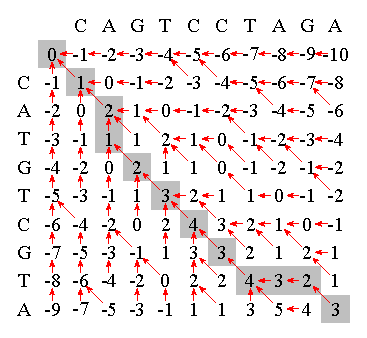
\includegraphics[width=\textwidth]{images/global_alignment}
    \end{subfigure}
    ~
    \begin{subfigure}[m]{0.3\textwidth}
    \centering
    \begin{verbatim}
    CATGTCAT--A
    CA-GTCCTAGA
    \end{verbatim}
    \end{subfigure}
    \caption[Tabuľka dyn. programovania pre  globálne zarovnanie]{Tabuľka dynamického programovania pre  globálne zarovnanie (vľavo) a výsledné zarovnanie (vpravo). Skóre je +1 za zhodu a -1 za nezhodu alebo medzeru.}
    \label{fig:global-align}
\end{figure}

Algoritmus postupne vypĺňa 2-rozmernú maticu $A$. Riadky zodpovedajú bázam sekvencie $X$ a stĺpce bázam $Y$. Na políčku $A[i,j]$ bude skóre najlepšieho zarovnania prvých $i$ báz sekvencie $X$ a prvých $j$ báz $Y$.

Keď zarovnávame sekvenciu s~prázdnou sekvenciou, tak skóre bude $-n$, kde $n$ je dĺžka sekvencie. Bude tam $n$ pomlčiek, každá nám dá skóre $-1$. Takto vyplníme riadky a stĺpce $A[i,0]$ a $A[0,j]$.

Ak chceme vyplniť políčko $A[i,j]$, musíme si uvedomiť ako môže vyzerať posledný stĺpec zarovnania $x_1x_2\dots x_i$ a $y_1y_2\dots y_j$. Máme iba 3 možnosti ako môže vyzerať posledný stĺpec najlepšieho zarovnania. Buď obsahuje $x_i$ alebo $y_j$ alebo oboje. V~prípade, že posledný stĺpec obsahuje oboje, cena tohto stĺpca je $s(x_i, y_j)$. Ak by sme posledný stĺpec zmazali, dostali by sme zarovnanie $x_1x_2\dots x_{i-1}$ a $y_1y_2\dots y_{j-1}$, pričom musí ísť o~najlepšie zarovnanie. To už máme vypočítané v~políčku $A[i-1, j-1]$, čiže výsledné skóre bude $A[i-1, j-1] + s(x_i,y_j)$.

V~prípade, že posledný stĺpec obsahuje len $x_i$ zarovnané s~pomlčkou, skóre stĺpca bude $-1$ a po zmazaní dostávame zarovnanie $x_1x_2\dots x_{i-1}$ a $y_1y_2\dots y_{j}$, výsledné skóre bude teda $A[i-1, j] -1$. V~prípade, že posledný stĺpec obsahuje len $y_i$, tak skóre vypočítame analogicky.

Najlepšie skóre bude maximálne skóre pre všetky 3 prípady.
Dostávame teda nasledujúci vzťah pre výpočet $A[i,j]$:
$$A[i,j] = \max \left\{
\begin{array}{l}
A[i-1,j-1]+s(x_i, y_j)\\
A[i-1,j]-d\\
A[i,j-1]-d
\end{array} \right.$$
Maticu vieme vypĺňať po riadkoch, pričom každé políčok vieme vypočítať z~troch políčok, ktoré už sú vypočítané. Políčko $A[0, 0] = 0$ a krajné políčka potom vieme vypočítať ako $A[i,0] = A[i-1,0]-d$ a $A[0, j] = A[0,j-1]-d$

Ak nás zaujíma aj zarovnanie -- nie len jeho skóre -- vieme si pre každé políčko zapamätať ktorá z~troch možností dosiahla maximálnu hodnotu
(červené šípky na obr. \ref{fig:global-align}). Na základe tejto informácie potom vieme zrekonštruovať zarovnanie tak, že postupne z~posledného políčka ($A[n,m]$) budeme prechádzať na políčko, z~ktorého sme vypočítali aktuálnu hodnotu.

Časová zložitosť je $O(nm)$, pretože vypĺňame $nm$ políčok, každé v~konštantnom čase. Zjavne aj pamäťová zložitosť je $O(nm)$.

Pamäťová zložitosť sa dá zredukovať na $O(n+m)$ za cenu zhruba dvojnásobného času výpočtu \cite{hirschberg}.

\subsection{Algoritmus pre lokálne zarovnanie: Smith-Waterman}

% TODO: preformulovať aby sedelo na lokalne zarovnania
%Máme dané 2 sekvencie $X = x_1x_2\dots x_n$ a $Y = y_1y_2\dots y_n$, budeme zarovnávať všetky znaky sekvencie $X$ a všetky znaky sekvencie $Y$. Budeme používať jednoduché skórovanie: $+1$ za zhodu, $-1$ za nezhodu alebo pomlčku.

\begin{figure}[htp]
    \centering
    \begin{subfigure}[m]{0.5\textwidth}
    \centering
    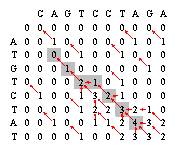
\includegraphics[width=\textwidth]{images/local_alignment}
    \end{subfigure}
    ~
    \begin{subfigure}[m]{0.3\textwidth}
    \centering
    \begin{verbatim}
    GT-CTA
    GTCCTA
    \end{verbatim}
    \end{subfigure}
    \caption[Tabuľka dyn. programovania pre  lokálne zarovnanie]{Tabuľka dynamického programovania pre  lokálne zarovnanie (vľavo) a výsledné zarovnanie (vpravo). Skóre je +1 za zhodu a -1 za nezhodu alebo medzeru.}
    \label{fig:local-align}
\end{figure}

Algoritmus pre lokálne zarovnania sa líši len v~niekoľkých malých detailoch. Opäť vypĺňame maticu $A$, s~tým, že v~$A[i,j]$ bude najvyššie skóre lokálneho zarovnania medzi sekvenciami $x_1x_2\dots x_i$ a $y_1y_2\dots y_j$, ktoré buď obsahuje bázy $x_i$ aj $y_j$, alebo je prázdne. Teda na ľubovoľnom mieste uvažujeme aj prázdne zarovnanie so skóre 0 (v~matici nebudú záporné čísla). Vzťah pre výpočet $A[i,j]$ vyzerá takto:
$$A[i,j] = \max \left\{
\begin{array}{l}
0\\
A[i-1,j-1]+s(x_i, y_j)\\
A[i-1,j]-d\\
A[i,j-1]-d
\end{array} \right.$$
V~tomto prípade sú všetky krajné políčka nulové.

Zarovnanie potom nájdeme tak, že začneme z~políčka s~maximálnym skóre, a postupne budeme prechádzať na políčka, z~ktorých sme získali maximálnu hodnotu, kým nenarazíme na nulu.

Časová aj pamäťová zložitosť sú, rovnako ako pri globálnom zarovnaní $O(nm)$.
\cite{durbin}

\subsection{Afínne skórovanie medzier}
\label{subsec:affine-gap-scoring}
V~jednoduchom skórovaní sme dávali za pomlčku vždy rovnaké skóre ($-1$). Pri evolúcii sa však môže stať, že sa naraz zmaže (alebo vloží) niekoľko susedných báz, čo je pravdepodobnejšie ako to, že sa dané bázy zmazali (alebo vložili) nezávisle. Pri \textit{afínnom skórovaní medzier} teda zavedieme dva typy skóre. Skóre za \textit{začatie medzery} a skóre za \textit{rozšírenie medzery}.

Algoritmus globálneho zarovnania vieme upraviť nasledovne: Namiesto matice $A$ teraz budeme mať 3 matice $M$, $I_x$, $I_y$ zodpovedajúce trom situáciám (obr. \ref{fig:affine-space-situations}).

\begin{figure}[htp]
    \centering
    \begin{subfigure}[m]{0.3\textwidth}
    \centering
    \begin{BVerbatim}[commandchars=\\\{\}]
    ACTx\textsubscript{i}
    AGTy\textsubscript{j}
    \end{BVerbatim}
    \caption{Mutácia($M$)}
    \end{subfigure}
    ~
    \begin{subfigure}[m]{0.3\textwidth}
    \centering
    \begin{BVerbatim}[commandchars=\\\{\}]
    ACTTAx\textsubscript{i}
    AGTy\textsubscript{j}--
    \end{BVerbatim}
    \caption{Inzercia v~X ($I_x$)}
    \end{subfigure}
    ~
    \begin{subfigure}[m]{0.3\textwidth}
    \centering
    \begin{BVerbatim}[commandchars=\\\{\}]
    ACTx\textsubscript{i}--
    AGTATy\textsubscript{j}
    \end{BVerbatim}
    \caption{Inzercia v~Y ($I_y$)}
    \end{subfigure}
    \caption[Situácie pri afínnoom skórovaní]{Tri situácie pri afínnoom skórovaní medzier}
    \label{fig:affine-space-situations}
\end{figure}

Nech $M[i,j]$ je najlepšie skóre prvých $i$ báz zo sekvencie $X$ a prvých $j$ báz zo sekvencie $Y$, pričom $x_i$ je zarovnané k~$y_j$, $I_x[i,j]$ je najlepšie skóre ak $x_i$ je zarovnané k~medzere a $I_y[i,j]$ je najlepšie skóre ak $y_j$ je zarovnané k~medzere.

Označme si $d$ penaltu za začatie medzery a $e$ penaltu za rozšírenie medzery. Vzťahy pre výpočet políčok sú nasledovné:
\begin{align*}
M[i,j] &= \max \left\{
\begin{array}{l}
M[i-1,j-1]+s(x_i, y_j)\\
I_x[i-1,j-1]+s(x_i, y_j)\\
I_y[i-1,j-1]+s(x_i, y_j)
\end{array} \right.\\
I_x[i,j] &= \max \left\{
\begin{array}{l}
M[i-1,j]-d\\
I_x[i-1,j]-e\\
I_y[i-1,j]-d
\end{array} \right.\\
I_y[i,j] &= \max \left\{
\begin{array}{l}
M[i,j-1]-d\\
I_x[i,j-1]-d\\
I_y[i,j-1]-e
\end{array} \right.
\end{align*}

V~týchto rovniciach predpokladáme, že delécia nie je nasledovaná inzerciou. Toto platí v~optimálnej sekvencii, ak $-d-s$ je menšie ako najmenšie skóre nezhody.

Tieto vzťahy vieme popísať stavovým diagramom na obrázku \ref{fig:alignment-fsa}:
\begin{figure}[h]
    \centering
    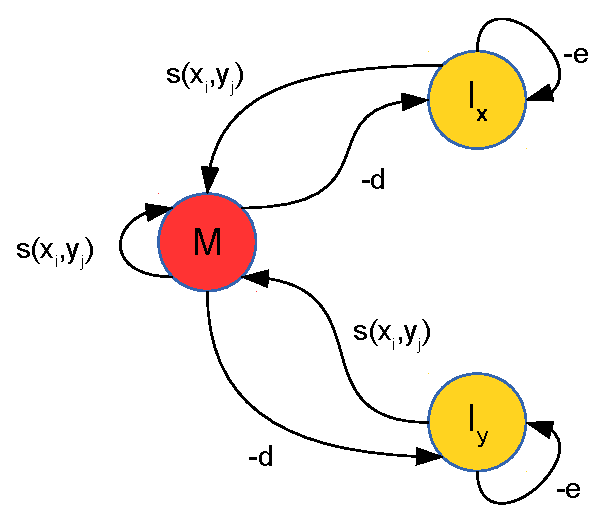
\includegraphics[width=.4\textwidth]{images/alignment_fsa}
    \caption[Stavový diagram pre zarovnanie sekvencií]{Stavový diagram pre zarovnanie sekvencií - obsahuje \textit{Match}~($M$), \textit{InsertX}~($I_x$) a \textit{InsertY}~($I_y$) stav a~prechody medzi nimi spolu s~ich cenou. Napríklad prechod z~$M$ do $I_x$ znamená vloženie medzery do $Y$-ovej sekvencie a to penalizujeme $-d$}
    \label{fig:alignment-fsa}
\end{figure}

Časová zložitosť je $O(nm)$, pretože vypĺňame $3nm$ políčok, každé v~konštantnom čase. Pamäťová zložitosť je opäť $O(nm)$.

\cite{durbin}

\section[Zarovnávanie s~pHMM]{Zarovnávanie pomocou skrytých Markovovských modelov}
\label{sec:hmm-alignment}

\textit{Skrytý markovovský model (Hidden Markov Model, HMM)} je generatívny pravdepodobnostný model, ktorý generuje náhodnú sekvenciu spolu s~jej anotáciou (stavmi). HMM sa podobá na konečný automat. Skladá sa z~konečného množstva stavov, prechodov medzi nimi a emisií.
V~každom kroku HMM vygeneruje a presunie sa do nejakého (aj toho istého) stavu. Generovanie symbolov aj presun medzi stavmi prebieha pravdepodobnostne.
% Na rozdiel od bežných konečných automatov, HMM emitujú symboly v~stave, nie počas prechodu.
% HMM sa skladá z~3 distribúcií
Konkrétny HMM je definovaný množinou stavov a nasledujúcimi distribúciami.
\begin{itemize}
\item distribúcia začiatočných stavov (pravdepodobnosť $\pi_i$, že HMM začne v~stave $i$)
\item distribúcia prechodov (pravdepodobnosť $a_{i,j}$, že HMM prejde zo stavu $i$ do stavu $j$)
\item distribúcia emisií (pravdepodobnosť $e_{i,x}$, že HMM v~stave $i$ vygeneruje symbol $x$)
\end{itemize}

Generovanie sekvencie teda vyzerá nasledovne: Na začiatku je HMM v~stave $i$ s~pravdepodobnosťou $\pi_i$. Potom v~každom kroku HMM emituje symbol $x$ s~pravdepodobnosťou $e_{i, x}$ a prejde do stavu $j$ s~pravdepodobnosťou $a_{i,j}$. Po $n$ krokoch takto vygenerujeme sekvenciu dĺžky $n$, pričom každý symbol je oanotovaný stavom, ktorý ho vygeneroval.

V~takomto modeli vieme počítať pravdepodobnosť, že model vygeneruje sekvenciu $x$ dĺžky $n$ s~anotáciou $s$ ako súčin pravdepodobností prechodov a emisií.
Výpočet vyzerá nasledovne:
$$P(X=x | S=s) = \pi_{s_1}\left(\prod_{i=1}^{n-1} e_{s_i,x_i} a_{s_i,s_i+1}\right)e_{s_n,x_n},$$
kde $x$ je postupnosť symbolov a $s$ je postupnosť stavov \cite{skripta, durbin}.


% % \subsection{Viterbiho algoritmus}
% % Hľadáme najpravdepodobnejšiu postupnosť stavov A, teda $\arg\max_A \Pr(A, S)$. Úlohu budeme riešiť dynamickým programovaním.

% % Podproblém $V[i,u]$ je pravdepodobnosť najpravdepodobnejšej cesty končiacej po $i$ krokoch v~stave $u$, pričom vygeneruje $s_1 s_2 \dots s_i$.

% % \begin{subequations}
% % Rekurentné vzťahy pre náš algoritmus sú nasledovné:
% % \begin{align}
% %         \label{eq:viterbi-init}
% %         V[1,u] &= \pi_u e_{s_1, u}\\
% %         \label{eq:viterbi-step}
% %         V[i,u] &= \max_w V[i-1, w] a_{w,u} e_{s_i, u}
% % \end{align}
% % \end{subequations}

% % Algoritmus funguje takto:
% % Nech $n$ je dĺžka reťazca a $m$ je počet stavov.

% % \begin{lstlisting}[escapechar=\%]
% % %Nainicializuj $V[1,i]\, \forall i$ podľa \ref{eq:viterbi-init}%
% % for i in range(2, n):
% %     for u~in range(1, m):
% %         %vypočítaj V[i, u] pomocou \ref{eq:viterbi-step}%
% % \end{lstlisting}
% % Maximálne V[n,j] je pravdepodobnosť najpravdepodobnejšej cesty
% % Aby sme vypísali anotáciu, pamätáme si pre každé V[i,u] stav w, ktorý viedol k~maximálnej hodnote vo vzorci \ref{eq:viterbi-step}.

% % Časová zložitosť tohto algoritmu je $O(nm^2)$, kde $n$ je dĺžka sekvencie a $m$ počet stavov.

% % Poznámka: pre dlhé sekvencie budú čísla V[i,u] veľmi malé a môže dôjsť k~podtečeniu. V~praxi teda používame zlogarimované hodnoty a namiesto násobenia súčet.

% \subsection{Nastavenie parametrov HMM}
% \label{subsec:hmmtraining}
% Ak máme oanotované trénovacie sekvencie, môžme z~nich parametre odvodiť frekvenčnou analýzou. Emisie získame tak, že vyfiltrujeme symboly s~príslušným stavom a spočítame frekvencie pre každý stav zvlášť a tranzície získame tak, že pre každý stav spočítame frekvencie nasledujúcich stavov. Tento postup sa volá \textit{metóda maximálnej vierohodnosti (v~angličtine maximum likelihood estimation)}. \cite{ durbin, wiki:mle}

\subsection{Zarovnávanie pomocou párových skrytých markovovských modelov (pHMM)}
\label{subsec:hmm-alignment}
% \todo mic odporúča rovno popísať párové hmm a aj viterbiho rovno naňom, takže to asi prepíšem

\textit{Párové skryté Markovovské modely (pHMM)} sa od tých obyčajných líšia v~tom, že namiesto jednej sekvencie generujú dvojicu sekvencií. Vedia generovať aj dvojicu symbolov aj jeden symbol v~jednej sekvencii a nula symbolov v~druhej. Na pHMM sa dajú použiť podobné algoritmy ako na HMM, ale treba ich upraviť tak, aby pracovali v~dvoch rozmeroch.

V~sekcii \ref{subsec:affine-gap-scoring} sme si ukázali jednoduchý algoritmus na globálne zarovnávanie s~afínnym skórovaním medzier. K~tomuto algoritmu sme si uviedli aj jednoduchý stavový automat (obr. \ref{fig:alignment-fsa}). Tento automat vieme previesť na pHMM.

Na to aby sme automat previedli na pHMM, musíme urobiť niekoľko zmien -- musíme nastaviť emisné a prechodové pravdepodobnosti, tak aby sčítavali do jedna.\cite{durbin}

\begin{figure}[htp]
    \centering
    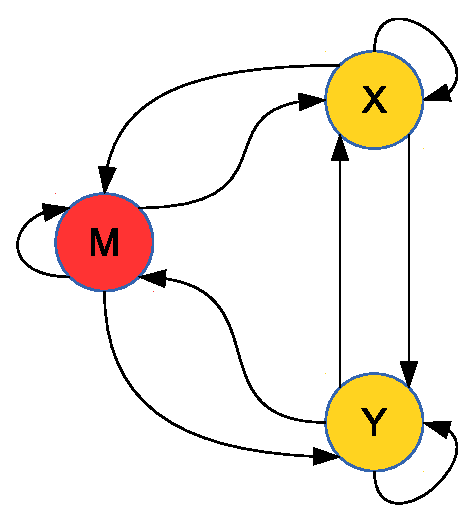
\includegraphics[width=.4\textwidth]{images/simple_model}
    \caption{Párový HMM pre zarovnávanie sekvencií}
    \label{fig:simple-model}
\end{figure}

\subsection{Viterbiho algoritmus na pHMM}
Hľadáme najpravdepodobnejšiu postupnosť stavov A~ak máme dané sekvencie $X$ a $Y$, teda $\arg\max_A \Pr(A, X, Y)$. Úlohu budeme riešiť dynamickým programovaním.

Podproblém $V[i, j, u]$ je pravdepodobnosť najpravdepodobnejšej postupnosti stavov končiacej v~$X[i]$ a $Y[j]$ v~stave $u$.

Inicializácia ($*$ označíme ľubovoľnú možnú hodnotu):
\begin{subequations}
\label{eq:viterbi-init}
\begin{align}
V[0,0,M] &= 1 \\
V[i,0,*] &= 0 \quad \forall i\\
V[0,j,*] &= 0 \quad \forall j
\end{align}
\end{subequations}

Rekurentné vzťahy:
\begin{subequations}
\label{eq:viterbi-rec}
\begin{align}
\label{eq:viterbi-recM}
V[i,j,M] &= e_{M, (x_i, y_j)} \max \left\{
\begin{array}{l}
a_{M,M} V[i-1,j-1,M]\\
a_{I_x,M} V[i-1,j-1,I_x]\\
a_{I_y,M} V[i-1,j-1, I_y]
\end{array} \right.\\
\label{eq:viterbi-recX}
V[i,j, I_x] &= e_{I_x, x_i}\max \left\{
\begin{array}{l}
a_{M, I_x} V[i-1,j,M]\\
a_{I_x, I_x} V[i-1,j,I_x]\\
a_{I_y, I_x} V[i-1,j,I_y]
\end{array} \right.\\
\label{eq:viterbi-recY}
V[i,j, I_y] &= e_{I_y, y_j}\max \left\{
\begin{array}{l}
a_{M, I_y} V[i,j-1,M]\\
a_{I_y, I_y} V[i,j-1,I_y]\\
a_{I_x, I_y} V[i,j-1,I_x]
\end{array} \right.
\end{align}
\end{subequations}

Algoritmus funguje takto:
Nech $n$ a $m$ sú dĺžky sekvencií $X$ a $Y$.
Na začiatku nainicializuje hodnoty pre $V[0,*,*]$ a $V[*,0,*]$ podľa \ref{eq:viterbi-init} ($*$ označíme ľubovoľnú možnú hodnotu).
Potom postupne pre všetky $i = 1\dots n$, $j = 1\dots m$ a $u \in \{M, I_x, I_y\}$ dynamicky vypočíta $V[i, j, u]$ podľa \ref{eq:viterbi-rec}.

Maximálne $V[n, m, u],\, \forall u \in \{M, I_x, I_y\}$ je pravdepodobnosť najpravdepodobnejšej postupnosti stavov.
Aby sme stavy vedeli zrekonštruovať, pamätáme si pre každé $V[i, j, u]$ stav $w$, ktorý viedol k~maximálnej hodnote. Táto postupnosť stavov nám udáva najpravdepodobnejšie zarovnanie.

Časová zložitosť tohto algoritmu je $O(nm)$.

Poznámka: pre dlhé sekvencie budú čísla $V[i, j, u]$ veľmi malé a môže dôjsť k~podtečeniu. V~praxi teda používame zlogaritmované hodnoty a namiesto násobenia súčet.
\cite{durbin}

\subsection{Nastavenie parametrov pHMM}
\label{subsec:hmmtraining}
Ak máme anotované trénovacie sekvencie, môžme HMM trénovať \textit{metódou maximálnej vierohodnosti (v~angličtine maximum likelihood estimation)}. \cite{ durbin, wiki:mle}
Emisie získame tak, že vyfiltrujeme symboly s~príslušným stavom a spočítame frekvencie pre každý stav zvlášť, pričom v~Match stave počítame frekvencie dvojíc symbolov. Tranzície získame tak, že pre každý stav spočítame frekvencie nasledujúcich stavov. Parametre modelu môžme teda ľahko natrénovať z~existujúcich párových zarovnaní.

\section[Štat. významnosť ]{Štatistická významnosť zarovnania}
Smith-Watermanov algoritmus nájde najlepšie lokálne zarovnanie pre ľubovoľné dve sekvencie. Treba však rozhodnúť, či je zarovnanie dostatočne vierohodné nato, aby predstavovalo skutočnú podobnosť sekvencií a nie len najlepšie zarovnanie dvoch nesúvisiacich sekvencií.
Ako vodítko pri rozhodnutí sa používajú identifikátory \textit{štatistickej významnosti} zarovnania: \textit{P-hodnota (P-value)} alebo \textit{E-hodnota (E-value)}.

\begin{figure}[htp]
    \centering
    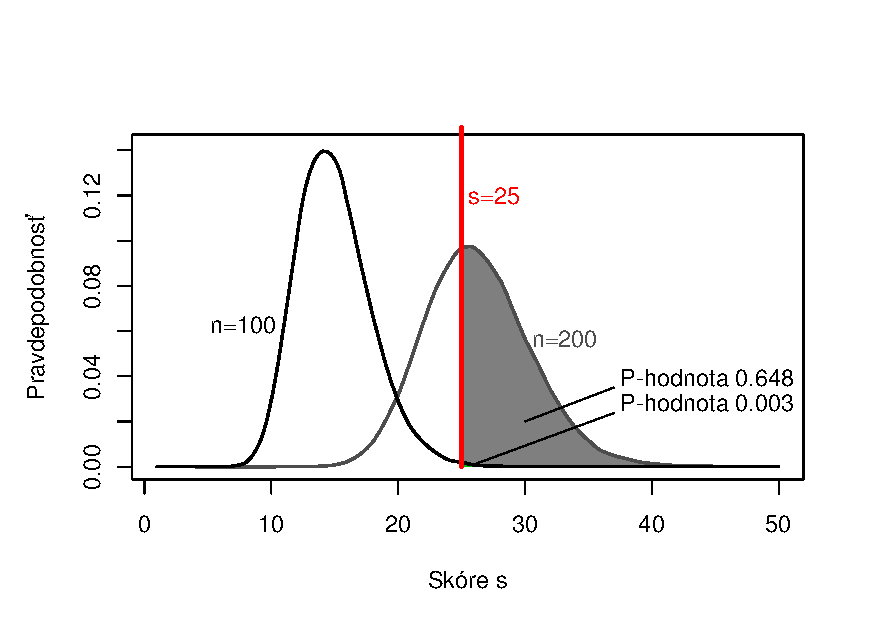
\includegraphics[width=.9\textwidth]{images/p-value}
    \caption[P-hodnota lokálneho zarovnania]{P-hodnota lokálneho zarovnania so skóre $s = 25$ medzi 2 sekvenciami dĺžky $n = 100$ alebo $n = 200$ (skórovanie $+1$ zhoda, $-1$ nezhoda alebo medzera). Rozdelenie bolo získané zarovnávaním $100000$ párov náhodných sekvencií. Pri $n=100$ je P-hodnota približne 0.003 a zodpovedá malej čiernej ploche pod krivkou napravo od zvislej čiary pre $s=25$. Pri dlhších sekvenciách zodpovedá P-hodnota veľkej sivej ploche napravo od zvislej čiary. Pri takto dlhých sekvenciách očakávame skóre 25 alebo väčšie vo viac ako 60\% prípadov čisto náhodou. Nejde teda o~štatisticky významné zarovnanie.}
    \label{fig:p-value}
\end{figure}

P-hodnota zarovnania je pravdepodobnosť, že medzi náhodne generovanými sekvenciami tej istej dĺžky by sme našli zarovnanie s~rovnakým skóre alebo vyšším. Keďže P-hodnota závisí od dĺžok sekvencií a skóre, musíme ju počítať pri každom zarovnaní. Je však časovo náročné robiť to generovaním veľkého množstva zarovnaní, preto sa používajú matematicky odvodené vzorce na odhad tejto hodnoty. (\cite{Karlin}, \cite{Mitrophanov}).

E-hodnota vyjadruje strednú hodnotu počtu zarovnaní so skóre aspoň takým ako má naše zarovnanie medzi náhodne generovanými sekvenciami. E-hodnota teda môže byť aj väčšia ako jedna. Ak je E-hodnota väčšia ako jedna, tak čisto náhodou by sme očakávali aspoň jedno také silné zarovnanie, a teda zarovnania s~takouto (a nižšou) E-hodnotou nebudeme považovať za štatisticky významné.

V~štatistike sa v~rôznych testoch štandardne používajú prahy na P-hodnotu $0.05$ alebo $0.01$.
Pri zarovnávaní sekvencií však často používame ešte nižší prah, teda uvažujeme len zarovnania s~P-hodnotou menšou ako napr. $10^{-5}$. Pri malých hodnotách sú P-hodnota a E-hodnota približne rovnaké, teda taký istý prah môžme použiť aj na E-hodnotu.

\input suvisiace_prace.tex
